\documentclass[12pt]{article}
\usepackage{amsmath, amsfonts, amsthm, amssymb}
\usepackage{fullpage}
\usepackage{enumerate}
\usepackage{hyperref}
\usepackage{multirow}

% For figures
\usepackage{graphicx}
\usepackage{subcaption}

% For code
\usepackage{listings}
% \renewcommand{\cftsecfont}{\rmfamily\mdseries\upshape}
% \renewcommand{\cftsecpagefont}{\rmfamily\mdseries\upshape} % No bold!
 \lstset{ 
  language=R,                     % the language of the code
  basicstyle=\footnotesize\ttfamily, % the size of the fonts that are used for the code
  numbers=none,                   % where to put the line-numbers
  backgroundcolor=\color{white},  % choose the background color. You must add \usepackage{color}
  showspaces=false,               % show spaces adding particular underscores
  showstringspaces=false,         % underline spaces within strings
  showtabs=false,                 % show tabs within strings adding particular underscores
  frame=single,                   % adds a frame around the code
  rulecolor=\color{black},        % if not set, the frame-color may be changed on line-breaks within not-black text (e.g. commens (green here))
  tabsize=2,                      % sets default tabsize to 2 spaces
  captionpos=b,                   % sets the caption-position to bottom
  breaklines=true,                % sets automatic line breaking
  breakatwhitespace=false,        % sets if automatic breaks should only happen at whitespace
  keywordstyle=\color{blue},      % keyword style
  commentstyle=\color{green},   % comment style
  stringstyle=\color{red}      % string literal style
} 

%%%%%%%%%%%%%%%%%%%%CONTENT MACROS%%%%%%%%%%%%%%%%%%%%%%%%%
\renewcommand{\qed}{\quad \ensuremath{\blacksquare}}    % QED blacksquare
\newcommand{\inv}{^{-1}}                            % inverse operator
\newcommand{\sminus}{\backslash}                    % set minus
\newcommand{\N}{\mathbb{N}}                         % natural numbers
\newcommand{\R}{\mathbb{R}}                         % real numbers
\newcommand{\pow}{\mathcal{P}}                      % power set
\newcommand{\Se}{\mathcal{S}}                       % partition
\newcommand{\D}{\mathcal{D}}                        % partition
\newcommand{\e}{\varepsilon}                        % \varepsilon
\renewcommand{\d}{\delta}                           % \delta
\newcommand{\X}{\mathcal{X}}                        % X domain
\newcommand{\Y}{\mathcal{Y}}                        % Y domain
\newcommand{\Z}{\mathcal{Z}}                        % Z domain
\newcommand{\A}{\mathcal{A}}                        % sub-domain
\newcommand{\E}{\mathbb{E}}                         % expected value
\newcommand{\V}{\mathbb{V}}                         % variance
\newcommand{\pr}{\mathbb{P}}                        % probability
\newcommand{\hP}{{\hat P}}                          % 
\newcommand{\cpest}{\widehat{p}_h}                  % clipped estimated density
\newcommand{\cqest}{\widehat{q}_h}                  % clipped estimated density
\newcommand{\pest}{\widetilde{p}_h}                 % estimated density
\newcommand{\qest}{\widetilde{q}_h}                 % estimated density
\newcommand{\dist}{\operatorname{dist}}             % distance operator
\newcommand{\acro}[1]{\textsc{\MakeLowercase{#1}}}
\newcommand{\ol}{\overline}
\renewcommand{\hat}{\widehat}
%%%%%%%%%%%%%%%%%%%%%%%%%%%%%%%%%%%%%%%%%%%%%%%%%%%%%%%%%%%

\renewcommand{\thesubsection}{\arabic{subsection}}

\usepackage{natbib}
\usepackage[disable]{todonotes}

\begin{document}
\begin{center}
{\bf\Large 37-462/662 HW 04 Solutions}\\
Peter Elliott \& Shashank Singh\\
\end{center}

\subsection*{Problem 1}
\begin{enumerate}[(a)]
\item By some of the given facts,
\begin{align}
\notag
\hat Y
    = X (X^T X)\inv X^T Y
 &  = U D V^T (V D U^T U D V^T)\inv V D U^T Y   & (X = U D V^T)                     \\
\notag
 &  = U D V^T (V D^2 V^T)\inv V D U^T Y         & (U^T U = I)                       \\
\notag
 &  = U D V^T V D^{-2} V^T V D U^T Y            & \hspace{-10mm}((V D^2 V^T)\inv = V D^{-2} V^T)  \\
    \label{eq:LR}
 &  = \mbox{\fbox{$U U^T Y$.}}                  & \hspace{-10mm}(V^T V = D D^{-2} D = I)
\end{align}
TODO: Interpret this
\item Again, by some of the given facts,
\begin{align*}
\hat Y_{ridge}
 &  = X (X^T X + \lambda I)\inv X^T Y                                       \\
 &  = U D V^T (V D U^T U D V^T + \lambda I)\inv V D U^T Y   & (X = U D V^T) \\
 &  = U D V^T (V D^2 V^T + \lambda I)\inv V D U^T Y         & (U^T U = I)   \\
 &  = U D V^T (V D^2 V^T + \lambda VV^T)\inv V D U^T Y      & (I = V^T V)   \\
 &  = U D V^T \left( V (D^2 + \lambda I) V^T \right) \inv V D U^T Y
                                                            & (\text{factor $V$ and $V^T$})  \\
 &  = U D V^T V (D^2 + \lambda I)\inv V^T V D U^T Y
            & ((V (D^2 + \lambda I) V^T)\inv = V (D^2 + \lambda I)\inv V^T) \\
 &  = \mbox{\fbox{$U D (D^2 + \lambda I)\inv D U^T Y$.}}    & (V^T V = I)   \\
\end{align*}
\item 
\end{enumerate}

Since the diagonal matrix $D (D^2 + \lambda I)\inv D$ multiplies the
$j^{th}$row of its argument by $\frac{d_j^2}{d_j^2 + \lambda}$,
\begin{equation}
\hat Y_{ridge}
    = U D (D^2 + \lambda I)\inv D U^T Y
    = \sum_{j = 1}^p \frac{d_j^2}{d_j^2 + \lambda} \cdot u_j u_j^T y.
\label{eq:ridge}
\end{equation}
If $\lambda = 0$, then $\frac{d_j^2}{d_j^2 + \lambda} = 1$, and so
(\ref{eq:ridge}) reduces to (\ref{eq:LR}).

On the other hand, if $\lambda > 0$, then
$\frac{d_j^2}{d_j^2 + \lambda} \in [0,1)$, and so this scalar shrinks the
contribution of the $j^{th}$ column of $U$. As $d_j \to 0$,
$\frac{d_j^2}{d_j^2 + \lambda} \to 0$, while, as $d_j \to \infty$,
$\frac{d_j^2}{d_j^2 + \lambda} \to 1$.

Since $d_j^2$ is proportional to the variance in the direction $v_j$, we see
that ridge regression shrinks most in the directions in which $X$ does not vary
much. This make sense because it is difficult to accurately estimate the effect
of a direction without a good spread of predictor data along that direction
(e.g., in the extreme case, if all observations of a particular variable are
identical, then we cannot regress over that variable).

\subsection*{Problem 2}
\begin{enumerate}
\item The \texttt{x1} and \texttt{x2} coordinates form a spiral centered at
$0$. $y$ appears to increase radially outwards along the spiral.
\begin{figure}[ht]
\centering
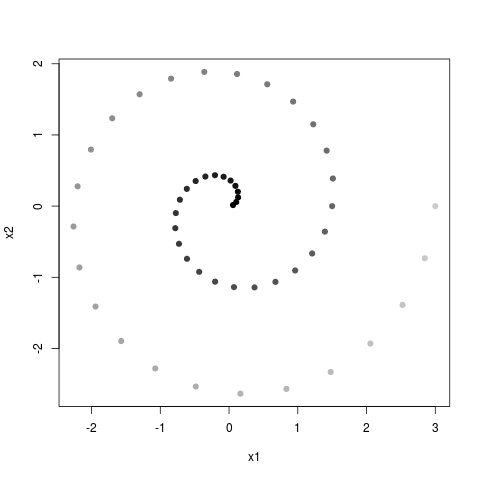
\includegraphics[width=0.7\textwidth]{2a}
\caption{Plot of \texttt{x1} and \texttt{x2}, colored by \texttt{y}.}
\label{fig:2a}
\end{figure}

\item 
\item 
\item 
\end{enumerate}

\subsection*{Problem 3}

\subsection*{Problem 4}

\subsection*{Code Appendix}
\subsubsection*{Problem 2}
\begin{lstlisting}
# part (a)
load('hw6spiral.RData')
plot(x1, x2, col = grey(0.8*(y - min(y))/(max(y) - min(y))), pch = 19)i
\end{lstlisting}


%{\small
%\bibliography{biblio}
%%\bibliographystyle{icml2014}
%\bibliographystyle{plain}
%}
\end{document}
